\documentclass{article}
\usepackage{graphicx}
\usepackage{amsmath}
\usepackage{pgfplots}
\usepackage{physics}
\usepackage{cancel}
\usepackage{enumitem}
\usepackage{txfonts}

\newcommand{\g}{\text{g}}
\newcommand{\kilo}{\text{k}}
\newcommand{\m}{\text{m}}
\newcommand{\centi}{\text{c}}
\newcommand{\s}{\text{s}}
\newcommand{\N}{\text{N}}
\newcommand{\J}{\text{J}}
\newcommand{\C}{\text{C}}
\newcommand{\V}{\text{V}}
\newcommand{\A}{\text{A}}
\newcommand{\Ohm}{\text{\Omega}}

\pgfplotsset{compat=1.18}

\usepackage[a4paper, top=1cm, bottom=2cm, left=2cm, right=2cm, includehead, includefoot]{geometry}

\begin{document}

\noindent
Physics 4B - Electromagnetism \hfill Prof. Alfred Cauthen

\noindent\rule{\textwidth}{0.4pt}

\begin{center}
    \textbf{\LARGE Homework 4} \\
    \vspace{12pt}
    \large Aaron W. Tarajos \\
    \textit{\today}
\end{center}

\noindent\rule{\textwidth}{0.4pt}

\section*{Chapter 22 Problem 50}
At some instant the velocity components of an electron moving between two charged parallel plates are $v_x=1.5 \times 10^5$ m/s and $v_y = 3.0 \times 10^3$ m/s. Suppose the electric field between the plates is uniform and given by $\vec{E} = 120$ N/C$\vu j$. In unit-vector notation, what are (a) the electron's acceleration in that field and (b) the electron's velocity when its $x$ coordinate has changed by 2.0 cm?

\subsection*{Solution}
\textbf{Part a:} There is only a force in the $\vu j$ direction and using Newton's second law we can say
\[
	\vec a = \frac{\vec F}{m} = \frac{120}{9.109 \times 10^{-31}} \frac{\N}{\C\ \kilo\g} = \boxed{1.317\times10^{32}\ \m/\s \ \vu j} 
\]
\textbf{Part b:} We can solve for time in terms of $v_x$;
\[
	\Delta x = v_xt \implies t = \frac{\Delta x}{v_x}
\]
then the velocity is given by;
\begin{align*}
	\vec v &= v_x\ \vu i + (at + v_y)\ \vu j \\
		   &= v_x\ \vu i + (\frac{a\Delta x}{v_x} + v_y)\ \vu j \\
		   &= 1.5 \times 10^5\ \m/\s \ \vu i + \frac{120 \cdot 2}{9.109 \times 10^{-31} \cdot 3.0 \times 10^3}\ \m/\s \ \vu j \\
		   &= \boxed{1.5 \times 10^5\ \m/\s \ \vu i + 8.783 \times 10^{28}\ \m/\s \ \vu j}
\end{align*}

\section*{Chapter 22 Problem 55}
A uniform electric field exists in a region between two oppositely charged plates. An elecctron is released from rest at the surface of the negatively charged plate and strikes the surface of the opposite plate, 2.0 cm away, in a time $1.5 \times 10^{-8}$ s. (a) What is the speed of the electron as it strikes the second plate? (b) What is the magnitude of the electric field $\vec{E}$?

\subsection*{Solution}
\textbf{Part a:}

\[
	a = \frac{2\Delta x}{t^2}
\]
and

\[
	v_f = v_i + at \implies v_f = \frac{2\Delta x}{t} 
\]
so we have

\[
	v_f = \frac{2\cdot 2.0}{1.5 \times 10^{-8}} = \boxed{2.667 \times 10^6\ \centi\m}
\]
\textbf{Part b:} We can use Newton's second law where
\begin{align*}
	F &= m a \\
	E &= m a \\
	&= m \frac{2\Delta x}{t^2} \\
	&= \frac{9.109 \times 10^{-31} \cdot 2 \cdot 0.02}{1.5 \times 10^{-16}} \\
	&= \boxed{2.430\times10^{-16} \ \N/\C}
\end{align*}

\section*{Chapter 22 Problem 59}
How much work is required to turn an electric dipole $180^\circ$ in a uniform electric field of magnitude $E = 46.0$ N/C if the dipole moment has a magnitude of $p=3.02 \times 10^{-25}\ \C \cdot \m$ and the initial angle is $64^\circ$?

\subsection*{Solution}
We start by finding the potential at the initial and final position and then take the difference between initial and final;
\[
	V = - \vec p \cdot \vec E
\]
and
\[
	W = -\Delta V
\]
so we have
\begin{align*}
	W &= -\left(pE \cos(64+180) pE \cos(64) \right) \\
	  &= -\left(\left(3.02 \times 10^{-25}\right)\left( 46\right) \cos(64+180) - \left(3.02 \times 10^{-25}\right)\left( 46\right) \cos(64) \right) \\ 
	  &= \boxed{1.2180\times10^{-23}\ \J}
\end{align*}

\section*{Chapter 22 Problem 60}
A certain electric dipole is placed in a uniform electric field $\vec E$ of magnitude $40.0\ \N/\C$ Figure 22-63 gives the magnitude $\tau$ of the torque on the dipole versus the angle $\theta$ between the field $\vec E$ and the dipole moment $\vec p$. The vertical axis scale is set by $\tau_s = 100 \times 10^{-28}\ \N \cdot \m $ What is the magnitude of $\vec p$?

\begin{figure}[ht]
    \centering
    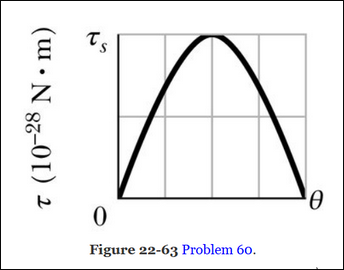
\includegraphics[scale=0.55]{image-1.png}
\end{figure}


\subsection*{Solution}
\[
	\vec \tau_s = \vec E \times \vec p \implies \tau_s = Ep\sin \theta
\]
we know that at $\theta = \frac{\pi}{2}$ that $\sin \theta = 1$ which is the maximum value and the graph seems to imply that is where the torque is equivalent to the scale. Therefore;
\begin{align*}
	\tau_{s,\text{max}} &= Ep \\
	p &= \frac{\tau_{s,\text{max}}}{E}   \\
	p &= \frac{100 \times 10^{-28}}{40.0} \frac{\N \cdot \m \cdot C}{\N}\\
	  &= \boxed{2.5\times10^{-28}\ \C \cdot \m}
\end{align*}

\section*{Chapter 22 Problem 76}
In Figure 22-67, an electric dipole swings from an initial orientation $\theta_1 = 20.0^\circ$ to a final orientation $\theta_2 = 20.0^\circ$ in a uniform external electric field $\vec E$. The electric dipole moment is $1.60 \times 10^{-27}\ \C \cdot \m$; the field magnitude is $3.00 \times 10^6\ \N/\C$. What is the change in the dipole's potential energy?

\begin{figure}[ht]
    \centering
    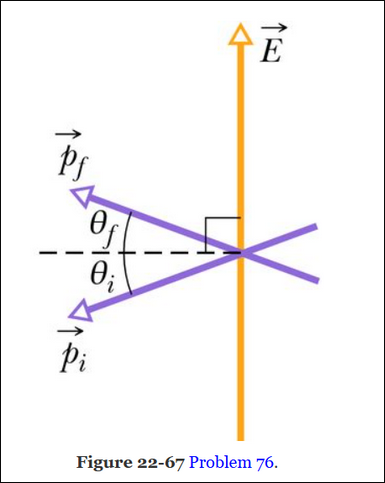
\includegraphics[scale=0.4]{image-2.png}
\end{figure}

\subsection*{Solution}
We just have to find the potential in both configurations and then take the difference,
\begin{align*}
	\Delta U &= Ep\cos(\theta_1) - Ep\cos(\theta_f) \\
			 &= 3.00 \times 10^6 \cdot 1.60 \times 10^{-27} \cdot \cos(70) - 3.00 \times 10^6 \cdot 1.60 \times 10^{-27} \cdot \cos(110) \\
			 &= \boxed{3.283\times10^{-21}\ \J}
\end{align*}

% \begin{figure}[ht]
%     \centering
%     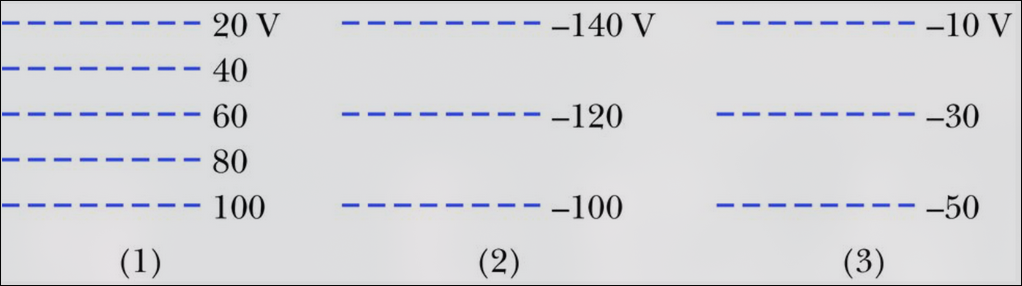
\includegraphics[scale=0.75]{image.png}
% \end{figure}

\end{document}
